

%******************************************************************************
% *filename:		02RequirementsDocument.tex
% *author:  		synckey
% *version: 		v1.0
% *datetime:		2011-04-22 20:50:49
% *description:
% *****************************************************************************/
\documentclass[12pt, a4paper, titlepage]{article}
\usepackage{fontspec}
\usepackage{graphicx}
\usepackage{float}
\usepackage{enumerate}
\usepackage{booktabs, multirow}
\usepackage[pagestyles]{titlesec}
\usepackage{xeCJK}
\renewcommand{\today}{\number\year-\number\month-\number\day}
\setmainfont[BoldFont=SimHei]{SimSun}
\setmonofont{SimSun}
\XeTeXlinebreaklocale"zh"
\title{DNS缓存系统软件需求规格说明书 }
\newpagestyle{mypagestyle}{
	\sethead{\sectiontitle}{}{$\cdot$~\thepage~$\cdot$
	}
	\setheadrule{1pt}
	\setfoot{}{}{\headrule}
}
\renewcommand{\contentsname}{目\quad 录}
\renewcommand{\figurename}{图}
\pagestyle{mypagestyle}
\makeatletter
\let\@afterindentfalse\@afterindenttrue
\@afterindenttrue
\makeatother
\setlength{\parindent}{2em}%中文缩进两个汉字位
\linespread{1.25}
\usepackage[colorlinks, linkcolor = blue , urlcolor = blue]{hyperref}
\begin{document}
\maketitle
\tableofcontents
\newpage

\section{ 概述 }

\subsection{编写目的}
	\indent
	本文档是李琳小组按DNS缓存项目需求的编制的。本文档的编写为下阶段的设计、开发提
	供依据,为项目组成员对需求的详尽理解,以及在开发开发过程中的协同工作提供强有力
	的保证。同时本文档也作为项目评审验收的依据之一。

\subsection{系统目标}
	\indent
	\textbf{场景描述:}在百度的大规模集群环境中,有这样一个模块,在它工作时,需要根据
	用户指定的机器名列表,与这些机器建立连接完成一定任务。在这个过程中,会大
	量进行域名的解析,不仅对DNS服务器造成较大压力,还容易发生解析失败的情况
	,设计一个系统,来应对突发性的、海量的DNS请求并在超出能力极限的情况下自我保护。
	该系统同时可以应用于短连接大并发的DNS请求并在超出能力极限的情况下自我保护。


\section{任务概述}
\subsection{目标}
\indent	本系统为其它系统服务,根据客户提出的域名,返回域名对应的IP地址。用户
	可以一次提出一个请求,也可以在一个请求中请求若干域名的IP地址。系统根据
	用户的请求,从DNS服务器获得域名和IP地址的对应关系,并进行缓存,从而在用户下
	次请求时,可以快速响应。当服务器的缓放满之后,就使用LIRS算法,对缓冲区进
	行更新。
	
\subsection{开发时限}
\indent 开发周期为25天,最后提交期限为2011年7月12号。
\section{系统需求说明}
\subsection{系统边界}

\begin{figure}[H]
\centering
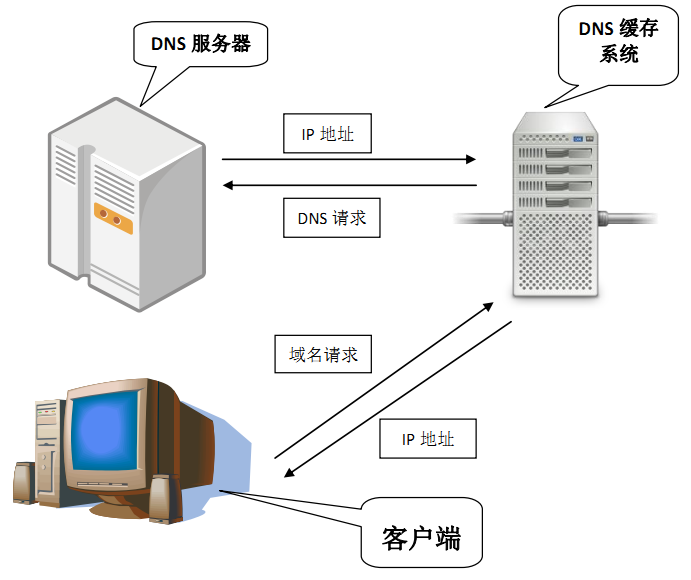
\includegraphics[keepaspectratio, scale=0.6]{pitures/dnsxitongbianjie.png}
\caption{系统边界}
\end{figure}

\subsection{功能需求}
\begin{enumerate}

	\item{可配置的缓存更新策略,如缓存的老化周期,缓存的大小。根据LIRS来实现
	缓存更新算法,并可扩展。}
	\item{处理网络请求,请求内容为一个或者n个主机名,返回对应的ip地址。包格
	式请考虑以后的扩展性。}
	\item{利用多核CPU,采用多线程实现。}
	\item{输入/输出:客户端的请求作为输入(其中包含请求所域名的计数以及每个请求域名的长度、请求内容),
	系统根据是否能在缓存中直接命中将输出分为两部分:可快速响应并返回给给客户端的输出,需要请求DNS
	服务器并返回的输出。}
	
\end{enumerate}
\subsection{性能需求}
\begin{enumerate}

	\item{在8*2.33G CPU,16G内存,64位主机上处理速度需要达到5000req/s。此数值将根
	据具体主机的不同而调整,基本评判标准是在相同缓存策略下,处理速度越快越好
	。}
	\item{对于超出系统承受能力的请求,使用拒绝策略来减少对正常服务的提供的影
	响。}
\end{enumerate}
\subsection{实现要求}
\begin{enumerate}
	\item{ 文档齐全:设计文档、单元测试文档、自动测试文档。文档的撰写思路明
	晰,内容完善。}
	\item{设计方面考虑完整,模块划分清晰。}
	\item{使用C实现。实现功能完整,代码符合代码规范,好的代码的可读性和
	可维护性,必要的注释。}
	\item{ 执行单元测试。}
	\item{ 完善的自动化测试用例。撰写程序对整体功能进行测试。}
\end{enumerate}
\subsection{安全性}
	保证服务器数据安全,不受DDoS攻击。
\section{功能划分}
%\subsection{主线程}
%主线程负责整个系统的调度。它接受客户的连接,在连接完成后,根据客户请求域名的数目
%以及线程池中空闲线程数目调度,每个线程完成一个域名的查找工作。
%\subsection{工作线程}
%工作线程完成一个域名和对应IP的查找工作,它从DNS获得IP,根据它自己的偏移,把结果
%写入要构建的发送给客户的应答报文中。各个工作线程协同完成客户的一次请求。
%\subsection{发送线程}
%发送线程分两次向客户


\subsection{内存管理模块}
给返回报文预分配内存,因此需要内存管理模块,进行预分配内存的管理,碎片整理,和防
止内存泄漏。。
\subsection{缓存管理模块}
本系统将从DNS服务器获取的域名和IP地址的对应关系缓存在内存中,采用LIRS算法驱动的缓存管理,提高缓存命中率。
\subsection{线程池管理及线程调度模块}
系统在启动时,预先分配固定数目的线程,放入线程池。当有客户连接请求域名时,从线程池中申请空闲线程,
线程工作完毕后将线程放回线程池中。
\subsection{通信协议}
指定客户端与系统的通信协议并使用协议通信。
\subsection{安全模块}
预防DDoS攻击。
\subsection{并发访问和同步机制}
线程间数据并发访问处理,和线程间的同步机制。
\subsection{客户端}
编写测试客户端,遵从通信协议协议与系统交互,客户端发送DNS解析请求并接收和处理服
务器的返回报文。
\subsection{自动化测试}
编写自动化测试客户端,测试系统的功能性需求和非功能性需求。

\section{验收标准}
\subsection{验收标准}
	\begin{itemize}
		\item{实现所有功能需求 }
		\item{满足非功能性需求 }
	  	\item{系统设计文档完整,且符合规范 }
	  	\item{代码符合规范,且与系统设计一致}
	\end{itemize}

\end{document}
%*********************************  END OF report.tex  *********************************/
